\documentclass{article}
\usepackage{graphicx} 
\usepackage{listings}

\begin{document}

\title{TCP File Transfer Protocol}
\author{Do Trong Dat - 22BI13075}
\date{\today}

\maketitle

\begin{abstract}
A simple file transfer protocol implemented using TCP/IP sockets in C++. The server listens for incoming connections on a specified port and receives a file from the client. The client connects to the server and sends the file contents.
\end{abstract}

\section{Protocol Design}

The protocol follows a basic request-response pattern:

\subsection{Client}

The client follows the steps outlined below:

\begin{enumerate}
    \item Perform DNS resolution for the hostname through \texttt{gethostbyname()}.
    \item Handle errors in operations such as creating sockets, connecting, sending, and receiving data.
    \item Create a socket using \texttt{socket()} and connect to the server using \texttt{connect()}.
    \item Open and read a file in chunks using \texttt{fread()}.
    \item Send data in chunks using \texttt{send()}.
    \item Close file and socket after communication is complete.
\end{enumerate}


\subsection{Server}

The server follows these steps:

\begin{enumerate}
    \item Listens for incoming connections on port 8080.
    \item Accepts connections from clients.
    \item Receives file data in chunks using \texttt{recv()}.
    \item Writes the received data to a file (e.g., \texttt{test2.txt}).
    \item Closes all resources after the transfer is complete.
\end{enumerate}


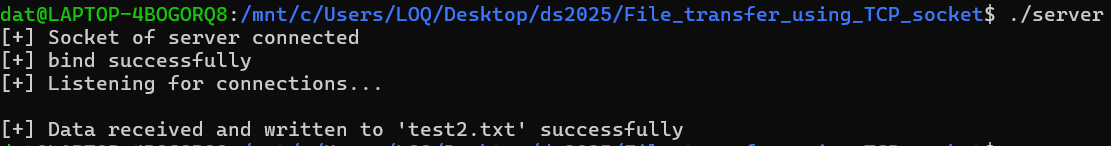
\includegraphics[width=1\linewidth]{image1.png}

\section{System Organization}

The system consists of two main components:

\subsection{Server}

The server listens for incoming connections on port 8080, receives file data in chunks, writes it to a file, and closes all resources after completion.
\begin{lstlisting}[language=C, caption=Sever C Code, label=lst:code]
#include <stdio.h>
#include <stdlib.h>
#include <string.h>
#include <sys/types.h>
#include <sys/socket.h>
#include <arpa/inet.h>
#include <unistd.h>
#include <fcntl.h>
#include <strings.h> // For bzero()

#define PORT 8080
#define SIZE 1024
#define LISTENQ 10 // Maximum number of pending connections

typedef struct sockaddr SA;

int open_listenfd(int port) {
    int listenfd, optval = 1;
    struct sockaddr_in serveraddr;

    if ((listenfd = socket(AF_INET, SOCK_STREAM, 0)) < 0) {
        perror("[-] Socket creation failed");
        return -1;
    }

    if (setsockopt(listenfd, SOL_SOCKET, SO_REUSEADDR, 
    (const void *)&optval, sizeof(int)) < 0) {
        perror("[-] Set socket options failed");
        return -1;
    }

    bzero((char *)&serveraddr, sizeof(serveraddr));
    serveraddr.sin_family = AF_INET;
    serveraddr.sin_addr.s_addr = htonl(INADDR_ANY);
    serveraddr.sin_port = htons((unsigned short)port);

    if (bind(listenfd, (SA *)&serveraddr, sizeof(serveraddr)) < 0) {
        perror("[-] Bind failed");
        return -1;
    }

    if (listen(listenfd, LISTENQ) < 0) {
        perror("[-] Listen failed");
        return -1;
    }

    return listenfd;
}

int main() {
    char buffer[SIZE];
    struct sockaddr_in clientaddr;
    socklen_t clientlen = sizeof(clientaddr);
    int listenfd, connfd, file_fd;

    listenfd = open_listenfd(PORT);
    if (listenfd < 0) {
        return 1; // Exit if server setup fails
    }
    printf("[+] Server is listening on port %d\n", PORT);

    connfd = accept(listenfd, (SA *)&clientaddr, &clientlen);
    if (connfd < 0) {
        perror("[-] Accept failed");
        close(listenfd);
        return 1;
    }
    printf("[+] Connection accepted\n");

    file_fd = open("test2.txt", O_WRONLY | O_CREAT | O_TRUNC, 0666);
    if (file_fd < 0) {
        perror("[-] Error opening/creating file");
        close(connfd);
        close(listenfd);
        return 1;
    }

    ssize_t bytes_received;
    while ((bytes_received = recv(connfd, buffer, SIZE, 0)) > 0) {  
    // Using recv()
        if (write(file_fd, buffer, bytes_received) != bytes_received) {
            perror("[-] Error writing to file");
            close(file_fd);
            close(connfd);
            close(listenfd);
            return 1;
        }
    }

    if (bytes_received < 0) {
        perror("[-] Error receiving data");
    }

    printf("[+] File received successfully\n");

    close(file_fd);
    close(connfd);
    close(listenfd);
    return 0;
}
\end{lstlisting}

\subsection{Client}

The client connects to the server, sends the filename, and transmits the file data in chunks.
\begin{lstlisting}[language=C, caption=Client C Code, label=lst:code]
#include <stdio.h>
#include <stdlib.h>
#include <string.h>
#include <sys/types.h>
#include <sys/socket.h>
#include <unistd.h>
#include <arpa/inet.h>
#include <netdb.h> // For gethostbyname()

#define PORT 8080
#define SIZE 1024

int open_clientfd(char *hostname, int port) {
    int clientfd;
    struct hostent *hp;
    struct sockaddr_in serveraddr;

    if ((clientfd = socket(AF_INET, SOCK_STREAM, 0)) < 0) {
        perror("[-] Socket creation failed");
        return -1;
    }

    if ((hp = gethostbyname(hostname)) == NULL) {
        perror("[-] DNS resolution failed");
        return -1;
    }

    bzero((char *)&serveraddr, sizeof(serveraddr));
    serveraddr.sin_family = AF_INET;
    bcopy((char *)hp->h_addr_list[0], (char *)
    &serveraddr.sin_addr.s_addr, hp->h_length);
    serveraddr.sin_port = htons(port);

    if (connect(clientfd, (struct sockaddr *)&serveraddr, 
    sizeof(serveraddr)) < 0) {
        perror("[-] Connection failed");
        return -1;
    }

    return clientfd;
}

int main() {
    char *hostname = "127.0.0.1"; // Replace with domain name if needed
    char buffer[SIZE];
    FILE *file;
    int clientfd;

    clientfd = open_clientfd(hostname, PORT);
    if (clientfd < 0) {
        return 1; // Exit if connection fails
    }
    printf("[+] Connected to server successfully\n");

    file = fopen("test.txt", "r");
    if (file == NULL) {
        perror("[-] Error opening file");
        close(clientfd);
        return 1;
    }

    ssize_t bytes_read, bytes_sent;
    while ((bytes_read = fread(buffer, 1, SIZE, file)) > 0) {
        bytes_sent = send(clientfd, buffer, bytes_read, 0); // Using send()
        if (bytes_sent < 0) {
            perror("[-] Error sending data");
            fclose(file);
            close(clientfd);
            return 1;
        }
    }

    printf("[+] File sent successfully\n");

    fclose(file);
    close(clientfd);
    return 0;
}

\end{lstlisting}
\begin{figure}
    \centering
    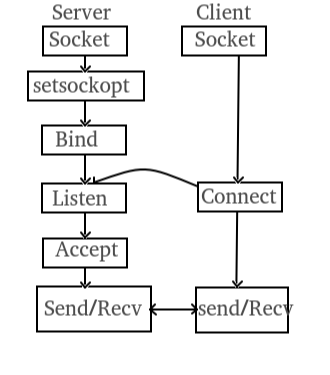
\includegraphics[width=1\linewidth]{Socket_server-1-modified.png}
    \caption{TCP file transfer flowchart}
    \label{fig:enter-label}
\end{figure}
\end{document}